\label{sec:part2_ablation}

A problem continuously mentioned throughout this report is Curse of Dimensionality. Undoubtedly, \texttt{KNN}, a distance–based ML method, suffers from it.
Nonetheless, tree–based models are less prone to this problem, on–going debates over tree models performance on high–dimensional data, though mostly favour feasibility of tree models when coping with high dimensionality \cite{JMLR:v18:16-466, 10.1007/978-3-031-80507-3_19, pmlr-v70-si17a, pmlr-v125-syrgkanis20a}.
We shall empricially challenge two viewpoints, by keeping and excluding the encoder, and later realise, either of which offer their own pros and cons. We present the results as below.
By the same caution raised in \textbf{Sec. \ref{sec:results_part2}}, \textbf{Protocol B} is slightly misleading due to data leakage.

We offer an additional table recording the time taken by classifiers in both training and testing.
\begin{table}[H]
    \centering
    \caption{\textbf{Protocol A} Held–out fitting and testing time (s).}
    \label{tab:time_compare}
    \begin{tabular}{ccccccc}
        \toprule
        Compressed? & \texttt{XGBoost} & \texttt{RF} & \texttt{CatBoost} & \texttt{AdaBoost} & \texttt{GBoost} & \texttt{KNN} \\
        \midrule
        No & 58.8 & 20.7 & 306.0 & 312.1 & 59.7 & 6.1 \\
        Yes & 0.8 & 1.5 & 6.1 & 2.9 & 5.3 & 0.2 \\
        \midrule
        \midrule
        Improved? & 73.5x & 13.8x & 50.2x & 107.6x & 11.3x & 30.5x \\
        \bottomrule
    \end{tabular}
\end{table}

Clearly, the total time taken to train and test the aforementioned classifiers substantially differ.
We further note that, for a trained \texttt{1D–CNN}–based extractor and \texttt{encoder}, the inference speed is not a bottleneck.

\begin{table}[H]
    \centering
    \caption{\textbf{Protocol B} class–wise performance metrics across models.}
    \label{tab:cv_classwise_part2_ablation}

    \begin{subtable}[t]{0.48\textwidth}
        \centering
        \caption{KNN}
        \label{tab:cv_knn_part2_ablation}
        \begin{tabular}{cccc}
            \toprule
            Class & Precision & Recall & F1 Score \\
            \midrule
            NORM (0) & 89.4 & 24.0 & 37.8 \\
            MI   (1) & 30.7 & 52.8 & 38.8 \\
            STTC (2) & 32.1 & 64.0 & 42.8 \\
            HYP  (3) & 15.7 & 57.7 & 24.5 \\
            CD   (4) & 41.4 & 65.4 & 50.6 \\
            \bottomrule
        \end{tabular}
    \end{subtable}
    \hfill
    \begin{subtable}[t]{0.48\textwidth}
        \centering
        \caption{Random Forest}
        \label{tab:cv_rf_part2_ablation}
        \begin{tabular}{cccc}
            \toprule
            Class & Precision & Recall & F1 Score \\
            \midrule
            NORM (0) & 83.5 & 84.6 & 84.1 \\
            MI   (1) & 65.6 & 59.9 & 62.6 \\
            STTC (2) & 63.0 & 65.0 & 63.9 \\
            HYP  (3) & 43.4 & 50.1 & 46.3 \\
            CD   (4) & 73.0 & 70.7 & 71.8 \\
            \bottomrule
        \end{tabular}
    \end{subtable}

    \bigskip

    \begin{subtable}[t]{0.48\textwidth}
        \centering
        \caption{Histogram–based Gradient Boosting}
        \label{tab:cv_gb_part2_ablation}
        \begin{tabular}{cccc}
            \toprule
            Class & Precision & Recall & F1 Score \\
            \midrule
            NORM (0) & 88.5 & 93.5 & 90.9 \\
            MI   (1) & 77.7 & 73.2 & 75.4 \\
            STTC (2) & 77.4 & 74.4 & 75.8 \\
            HYP  (3) & 64.8 & 49.9 & 56.0 \\
            CD   (4) & 84.8 & 77.7 & 81.0 \\
            \bottomrule
        \end{tabular}
    \end{subtable}
    \hfill
    \begin{subtable}[t]{0.48\textwidth}
        \centering
        \caption{AdaBoost}
        \label{tab:cv_ada_part2_ablation}
        \begin{tabular}{cccc}
            \toprule
            Class & Precision & Recall & F1 Score \\
            \midrule
            NORM (0) & 84.6 & 66.0 & 74.1 \\
            MI   (1) & 43.5 & 48.5 & 45.7 \\
            STTC (2) & 48.9 & 62.9 & 54.9 \\
            HYP  (3) & 24.9 & 59.1 & 34.8 \\
            CD   (4) & 51.8 & 59.5 & 55.0 \\
            \bottomrule
        \end{tabular}
    \end{subtable}

    \bigskip

    \begin{subtable}[t]{0.48\textwidth}
        \centering
        \caption{CatBoost}
        \label{tab:cv_cat_part2_ablation}
        \begin{tabular}{cccc}
            \toprule
            Class & Precision & Recall & F1 Score \\
            \midrule
            NORM (0) & 89.8 & 93.2 & 91.5 \\
            MI   (1) & 78.8 & 74.4 & 76.5 \\
            STTC (2) & 76.8 & 76.9 & 76.8 \\
            HYP  (3) & 63.6 & 53.8 & 57.8 \\
            CD   (4) & 82.6 & 77.2 & 79.8 \\
            \bottomrule
        \end{tabular}
    \end{subtable}
    \hfill
    \begin{subtable}[t]{0.48\textwidth}
        \centering
        \caption{XGBoost}
        \label{tab:cv_xgb_part2_ablation}
        \begin{tabular}{cccc}
            \toprule
            Class & Precision & Recall & F1 Score \\
            \midrule
            NORM (0) & 87.4 & 93.8 & 90.5 \\
            MI   (1) & 78.3 & 71.6 & 74.7 \\
            STTC (2) & 76.6 & 73.8 & 75.1 \\
            HYP  (3) & 63.6 & 45.4 & 52.8 \\
            CD   (4) & 84.6 & 74.6 & 79.2 \\
            \bottomrule
        \end{tabular}
    \end{subtable}
\end{table}

\begin{table}[H]
    \centering
    \caption{\textbf{Protocol B} Performance metrics across all models.}
    \label{tab:single_model_wise_part2_ablation}
    \begin{tabular}{ccccccc}
        \toprule
        Metrics & \texttt{XGBoost} & \texttt{RF} & \texttt{CatBoost} & \texttt{AdaBoost} & \texttt{GBoost} & \texttt{KNN} \\
        \midrule
        Precision & 78.1 & 65.7 & 78.3 & 50.7 & 78.6 & 41.9 \\
        Recall & 71.8 & 66.0 & 75.1 & 59.2 & 73.7 & 52.8 \\
        F1 Score & 74.5 & 65.7 & 76.5 & 52.9 & 75.8 & 38.9 \\
        Accuracy & $83.8$ & $75.3$ & $84.9$ & $61.9$ & $84.4$ & $39.9$ \\
        \midrule
        \midrule
        Time (s) & 647.0 & 246.1 & 2903.3 & 3493.7 & 646.5 & 28.2 \\
        \bottomrule
    \end{tabular}
\end{table}

Considering the tables above, removing the compression stage divides the classifiers.
Given all $2{,}225$ features, the boosted ensembles gain $17.0$–$18.7$ F1 points over \textbf{Tab. \ref{tab:single_model_wise_part2}}, \texttt{CatBoost} reaching $76.5$, while \texttt{RF} and \texttt{AdaBoost} gain $8.9$ and $8.7$.
\texttt{KNN} is the only model to deteriorate, from $47.9$ to $38.9$ F1, notably for NORM, its recall collapses to $24.0$, only $416$ of $1{,}791$ NORM records are recognised in \textbf{Fig. \ref{fig:part2_ablation_confusion}}.
Tree–based models thus exploit the high–dimensional input, whereas the distance–based \texttt{KNN} depends on compression.
The gain is costly, as fitting takes $12$–$106\times$ longer, e.g. $57.2 \rightarrow 2{,}903.3$\,s for \texttt{CatBoost}.

Looking at the single 80/20 held–out evaluation.
In \textbf{Fig. \ref{fig:part2_ablation_confusion}}, \texttt{XGBoost}, \texttt{GBoost} and \texttt{CatBoost} reach only $74.9$–$75.0\%$ accuracy, against $1.0$–$2.1$ for the remaining models here and $1.0$–$2.3$ in \textbf{Sec. \ref{sec:results_part2}}.
Even so, held–out accuracy still improves over the compressed pipeline by $8.3$–$10.1$ points for these three models and $7.5$ for \texttt{RF}, while \texttt{KNN} loses $17.1$.
Class–wise AUCs in \textbf{Fig. \ref{fig:part2_ablation_roc}} rise to $0.87$–$0.93$ for the ensembles, from $0.81$–$0.90$, and HYP becomes the lowest–scoring class for \texttt{XGBoost}, \texttt{GBoost} and \texttt{CatBoost}.

\begin{figure}[H]
    \centering
    \caption{\textbf{Protocol A} Confusion matrices of all classifiers.}
    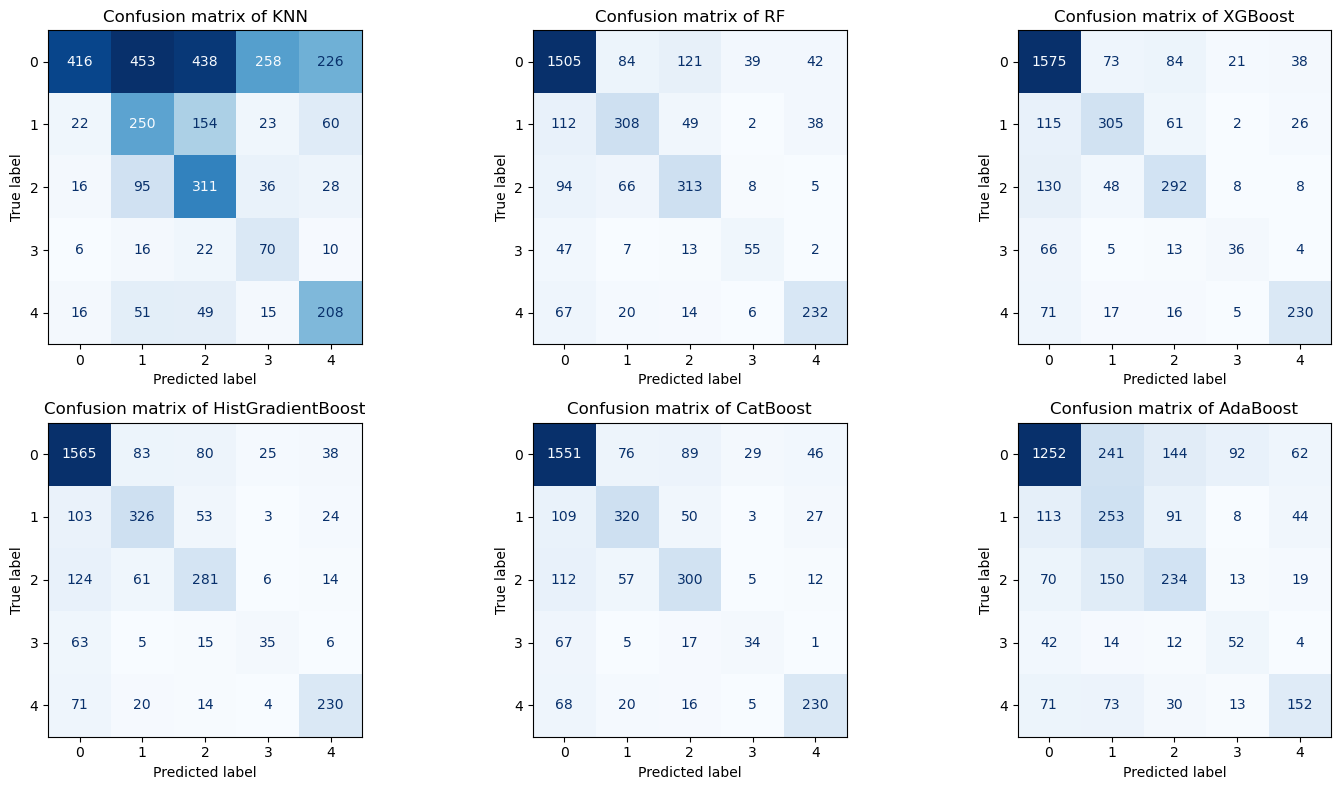
\includegraphics[width=\textwidth]{figures/part2/ablation_cm.png}
    \label{fig:part2_ablation_confusion}
\end{figure}

\begin{figure}[H]
    \centering
    \caption{\textbf{Protocol A} ROC–AUC curves and scores across classifiers.}
    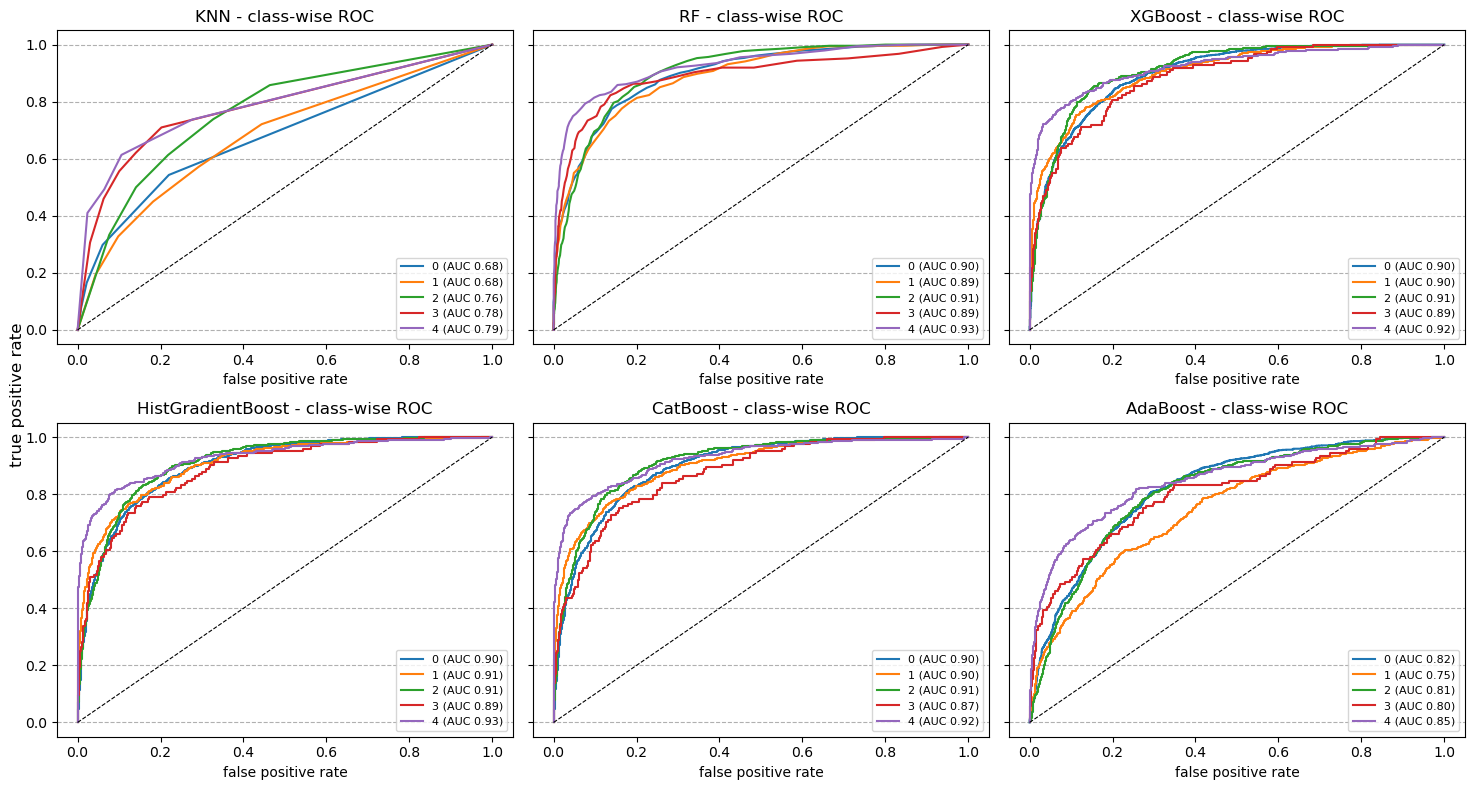
\includegraphics[width=\textwidth]{figures/part2/ablation_roc_curves.png}
    \label{fig:part2_ablation_roc}
\end{figure}
